% Section 5: Forecasting for RL -- the forecaster as policy (Story 2, part 2)
\subsection{Forecasting for RL: the forecaster as policy}
\label{sec:forecaster_as_policy}
\label{sec:forecasting_in_rl}

Section~\ref{sec:model_based_planning} kept the forecaster as a component
that feeds a separate planner or value function. This section takes the
inversion further. The forecaster is the agent. Two flavours matter for
the chapter, namely trajectory generative models that treat the policy as
a forecast over future state-action sequences and counterfactual
forecasters that estimate the value of an alternative policy from logged
trajectories.

\subsubsection{Trajectory generative models}
\label{sec:trajectory_gen}

An offline reinforcement-learning dataset is a collection of trajectories
$\tau = (s_0, a_0, r_0, s_1, a_1, r_1, \dots, s_T, a_T, r_T)$ generated by
some behaviour policy. A trajectory generative model treats $\tau$ as a
sequence and trains a generative model on those sequences. The
\citet{Chen2021DT} Decision Transformer represents each trajectory as a
flat sequence
\begin{equation}
\tau = (\widehat R_0, s_0, a_0,\, \widehat R_1, s_1, a_1,\, \dots,\,
  \widehat R_T, s_T, a_T),
\label{eq:dt_sequence}
\end{equation}
where $\widehat R_t = \sum_{t' \ge t} r_{t'}$ is the return-to-go from
time $t$ onwards. A causally masked GPT-style transformer is trained to
predict the next action token given the last $K$ context tokens. At test
time, the operator specifies a desired return $R^\star$ and primes the
model with $\widehat R_0 = R^\star$ and the current state $s_0$. The model
generates the corresponding action, the environment returns a reward and
the next state, the operator decrements $R^\star$ by the realised reward,
and the loop repeats. No value function, no policy gradient, no critic
appears in training. The forecaster is the policy.

The empirical case rests on D4RL and Atari. On the $1\%$ DQN-replay slice
of Atari, the Decision Transformer attains gamer-normalised scores of
$267.5$ on Breakout against the $211.1$ of Conservative Q-Learning, the
incumbent offline-RL baseline. On the D4RL locomotion benchmark, the
Decision Transformer averages $74.7$ across nine task-dataset
combinations against CQL's $54.2$ and behavioural cloning's
$47.7$.\footnote{The same trajectory-as-sequence reframing was independently
proposed by \citet{Janner2021TT}, with beam search over tokenised states
and actions replacing return conditioning. Subsequent diffusion variants
\citep{Janner2022diffuser,Ajay2023} replace autoregressive generation with
iterative denoising of an entire trajectory and dispense with dynamic
programming entirely. The methodological move is the same. Plan by
sampling from a generative model of structured objects rather than by
maximising a learned value function.} For economists familiar with
structural estimation, the conceptual draw is that a forecast distribution
over trajectories doubles as the policy itself. The conditioning variable
plays the role of a behavioural target rather than a payoff.

\subsubsection{Counterfactual forecasting for off-policy evaluation}
\label{sec:counterfactual_ope}

Off-policy evaluation asks the question every applied economist asks at
some point. Given a logged dataset generated by a behaviour policy
$\pi_{\mathrm{obs}}$, what would the return have been under an alternative
policy $\widetilde\pi$? Importance sampling estimators are unbiased under
common support but high variance. Model-based estimators are low variance
but biased by model misspecification. The counterfactual route of
\citet{Buesing2019} sits between the two.

The construction casts the partially observable Markov decision process as
a structural causal model. The transition mechanism is
$s_{t+1} = f^s(s_t, a_t, u^s_t)$ with exogenous noise $u^s_t$, the
observation mechanism is $o_t = f^o(s_t, u^o_t)$, and the action
mechanism is $a_t = f^\pi(h_t, u^a_t)$ given the history. Given an
observed trajectory $\hat\tau$, the counterfactual rule has three steps.

\begin{algorithm}[h]
\caption{Counterfactual off-policy evaluation \citep{Buesing2019}}
\label{alg:buesing_cfope}
\begin{algorithmic}[1]
\State \emph{Abduction.} Infer the posterior $P(U \mid \hat\tau)$ over the
exogenous noise from the observed trajectory.
\State \emph{Action.} Replace the behaviour-policy mechanism $f^\pi$ with
the target-policy mechanism $f^{\widetilde\pi}$ to form the modified SCM
$\mathcal M^{\mathrm{do}(\widetilde\pi)}_{\hat\tau}$ with the same posterior
on $U$.
\State \emph{Prediction.} Sample $U \sim P(U \mid \hat\tau)$ and roll out
the modified SCM to obtain counterfactual trajectories $\tau^{\mathrm{cf}}$
and their returns.
\end{algorithmic}
\end{algorithm}

Lemma~1 of \citet{Buesing2019} establishes that the marginal of the
counterfactual distribution over $\hat\tau$ equals the interventional
distribution. The counterfactual estimator is unbiased under correct SCM
specification. On the partially-observable grid-world experiment of the
paper, the counterfactual estimator's evaluation error decreases
monotonically with the amount of off-policy data, while the model-based
estimator's error remains stuck at the bias of the dynamics model.

The categorical-action case raises an identification problem.
\citet{Oberst2019} show that multiple structural causal models can be
consistent with the same interventional distribution yet imply different
counterfactual outcomes, and resolve the ambiguity by assuming a
Gumbel-max sampling mechanism that satisfies a counterfactual-stability
condition.\footnote{The Pearl monotonicity condition resolves the binary
case. The Gumbel-max SCM is the natural extension to $k$-way categorical
outcomes. \citet{TangWiens2023} combine SCM-based counterfactual outcomes
with importance sampling to obtain variance reductions while preserving
unbiasedness under correct human annotation, with a sepsis-simulator
demonstration that delivers an RMSE of $0.013$ against $0.113$ for vanilla
per-decision IS.} The shared identifying assumption across this strand is
that the structural causal model is correctly specified. The Lucas
critique applies in its sharpest form when the agent's policy itself
enters the data-generating process. Identification by instruments or by
exogeneity restrictions, in the spirit of \citet{Chernozhukov2018}, is the
econometric remedy and remains an open research question for the
counterfactual-RL programme. The full econometric identification toolkit
for sequential confounded settings, namely backdoor adjustment,
instrumental variables, proximal and partially-observed bridges, and
mediator-based identification, is developed in the chapter on causal
inference for reinforcement learning; the structural-causal-model
machinery of this subsection is its structural complement rather than its
substitute.

\subsubsection{Simulation: counterfactual OPE under a misspecified SCM}
\label{sec:cfope_sim}

A second synthetic instance illustrates the counterfactual machinery on a
substrate that mirrors the contextual-bandit reading of
Section~\ref{sec:counterfactual_ope}. The DGP is a linear structural
causal model in two features,
\begin{equation}
y = 1 + 0.5\, x_1 - 0.3\, x_2 + 2\, a + a \cdot x_1 + u,
\qquad u \sim \mathcal N(0,\, 0.5^2),
\label{eq:cfope_dgp}
\end{equation}
with $x \sim \mathcal N(0, I_2)$, a binary action $a \in \{0, 1\}$, and
a heterogeneous treatment effect $\tau(x) = 2 + x_1$. The behaviour
policy $\pi_{\mathrm{obs}}(a = 1 \mid x) = \sigma(0.5 + x_1 - 0.5\, x_2)$
is confounded with $x$. The target policy $\widetilde\pi(a \mid x) =
\mathbf 1\{x_1 + x_2 > 0\}$ is a deterministic threshold rule. The
oracle value $V(\widetilde\pi) = \mathbb E_x[y \mid a =
\widetilde\pi(x)]$ is computed by Monte Carlo at $10^6$ realisations.

Three estimators are compared on $n \in \{200, 500, 1000, 2000\}$ logged
samples, $20$ seeds per cell. Per-decision importance sampling is
$\widehat V_{\mathrm{IS}} = n^{-1} \sum_i \rho_i y_i$ with $\rho_i =
\mathbf 1\{a_i = \widetilde\pi(x_i)\} / \pi_{\mathrm{obs}}(a_i \mid
x_i)$. The model-based plug-in $\widehat V_{\mathrm{MB}} = n^{-1}
\sum_i \hat f(x_i, \widetilde\pi(x_i))$ uses an OLS fit $\hat f$ on the
logged data. The counterfactual estimator follows the Buesing
abduction-action-prediction rule and combines $\hat f$ with a
residual correction weighted by the importance ratio,
\begin{equation}
\widehat V_{\mathrm{CF}}
= n^{-1} \sum_i \hat f(x_i, \widetilde\pi(x_i))
  + n^{-1} \sum_i \rho_i \bigl(y_i - \hat f(x_i, a_i)\bigr),
\label{eq:cfope_dr}
\end{equation}
which is the doubly-robust form of the abduction-action-prediction rule
and is unbiased under correct propensity \emph{or} correct
model.\footnote{The naive average of the per-observation counterfactual
outcome $y'_i = \hat f(x_i, \widetilde\pi(x_i)) + (y_i - \hat f(x_i,
a_i))$ collapses to $\widehat V_{\mathrm{MB}}$ under OLS with an
intercept, because the OLS residuals sum exactly to zero. The
importance-weighted residual correction in \eqref{eq:cfope_dr} restores
the bias-cancellation property in finite samples. The estimator
coincides with the classical doubly-robust estimator of
Robins-Rotnitzky-Zhao adapted to off-policy evaluation.} The
well-specified scenario uses the feature set $\{1, x_1, x_2, a,
a \cdot x_1\}$ in $\hat f$, matching the DGP. The misspecified scenario
drops the interaction $a \cdot x_1$, the source of the heterogeneous
treatment effect.

\begin{table}[h]
\centering
\caption{Counterfactual off-policy evaluation under a linear SCM,
$n = 1000$, $20$ seeds. The CF estimator's residual correction cancels
the MB bias under misspecification while inheriting low variance from
the model.}
\label{tab:cfope_summary}
% Generated by counterfactual_ope.py
\begin{tabular}{llccc}
\hline\hline
Scenario & Estimator & Bias & Std & RMSE \\
\hline
Well-specified & IS & $+0.017$ & $0.100$ & $0.099$ \\
 & MB & $-0.001$ & $0.057$ & $0.056$ \\
 & CF & $+0.003$ & $0.067$ & $0.065$ \\
\hline
Misspecified & IS & $+0.017$ & $0.100$ & $0.099$ \\
 & MB & $-0.072$ & $0.061$ & $0.093$ \\
 & CF & $+0.002$ & $0.078$ & $0.076$ \\
\hline\hline
\end{tabular}

\end{table}

\begin{figure}[h]
\centering
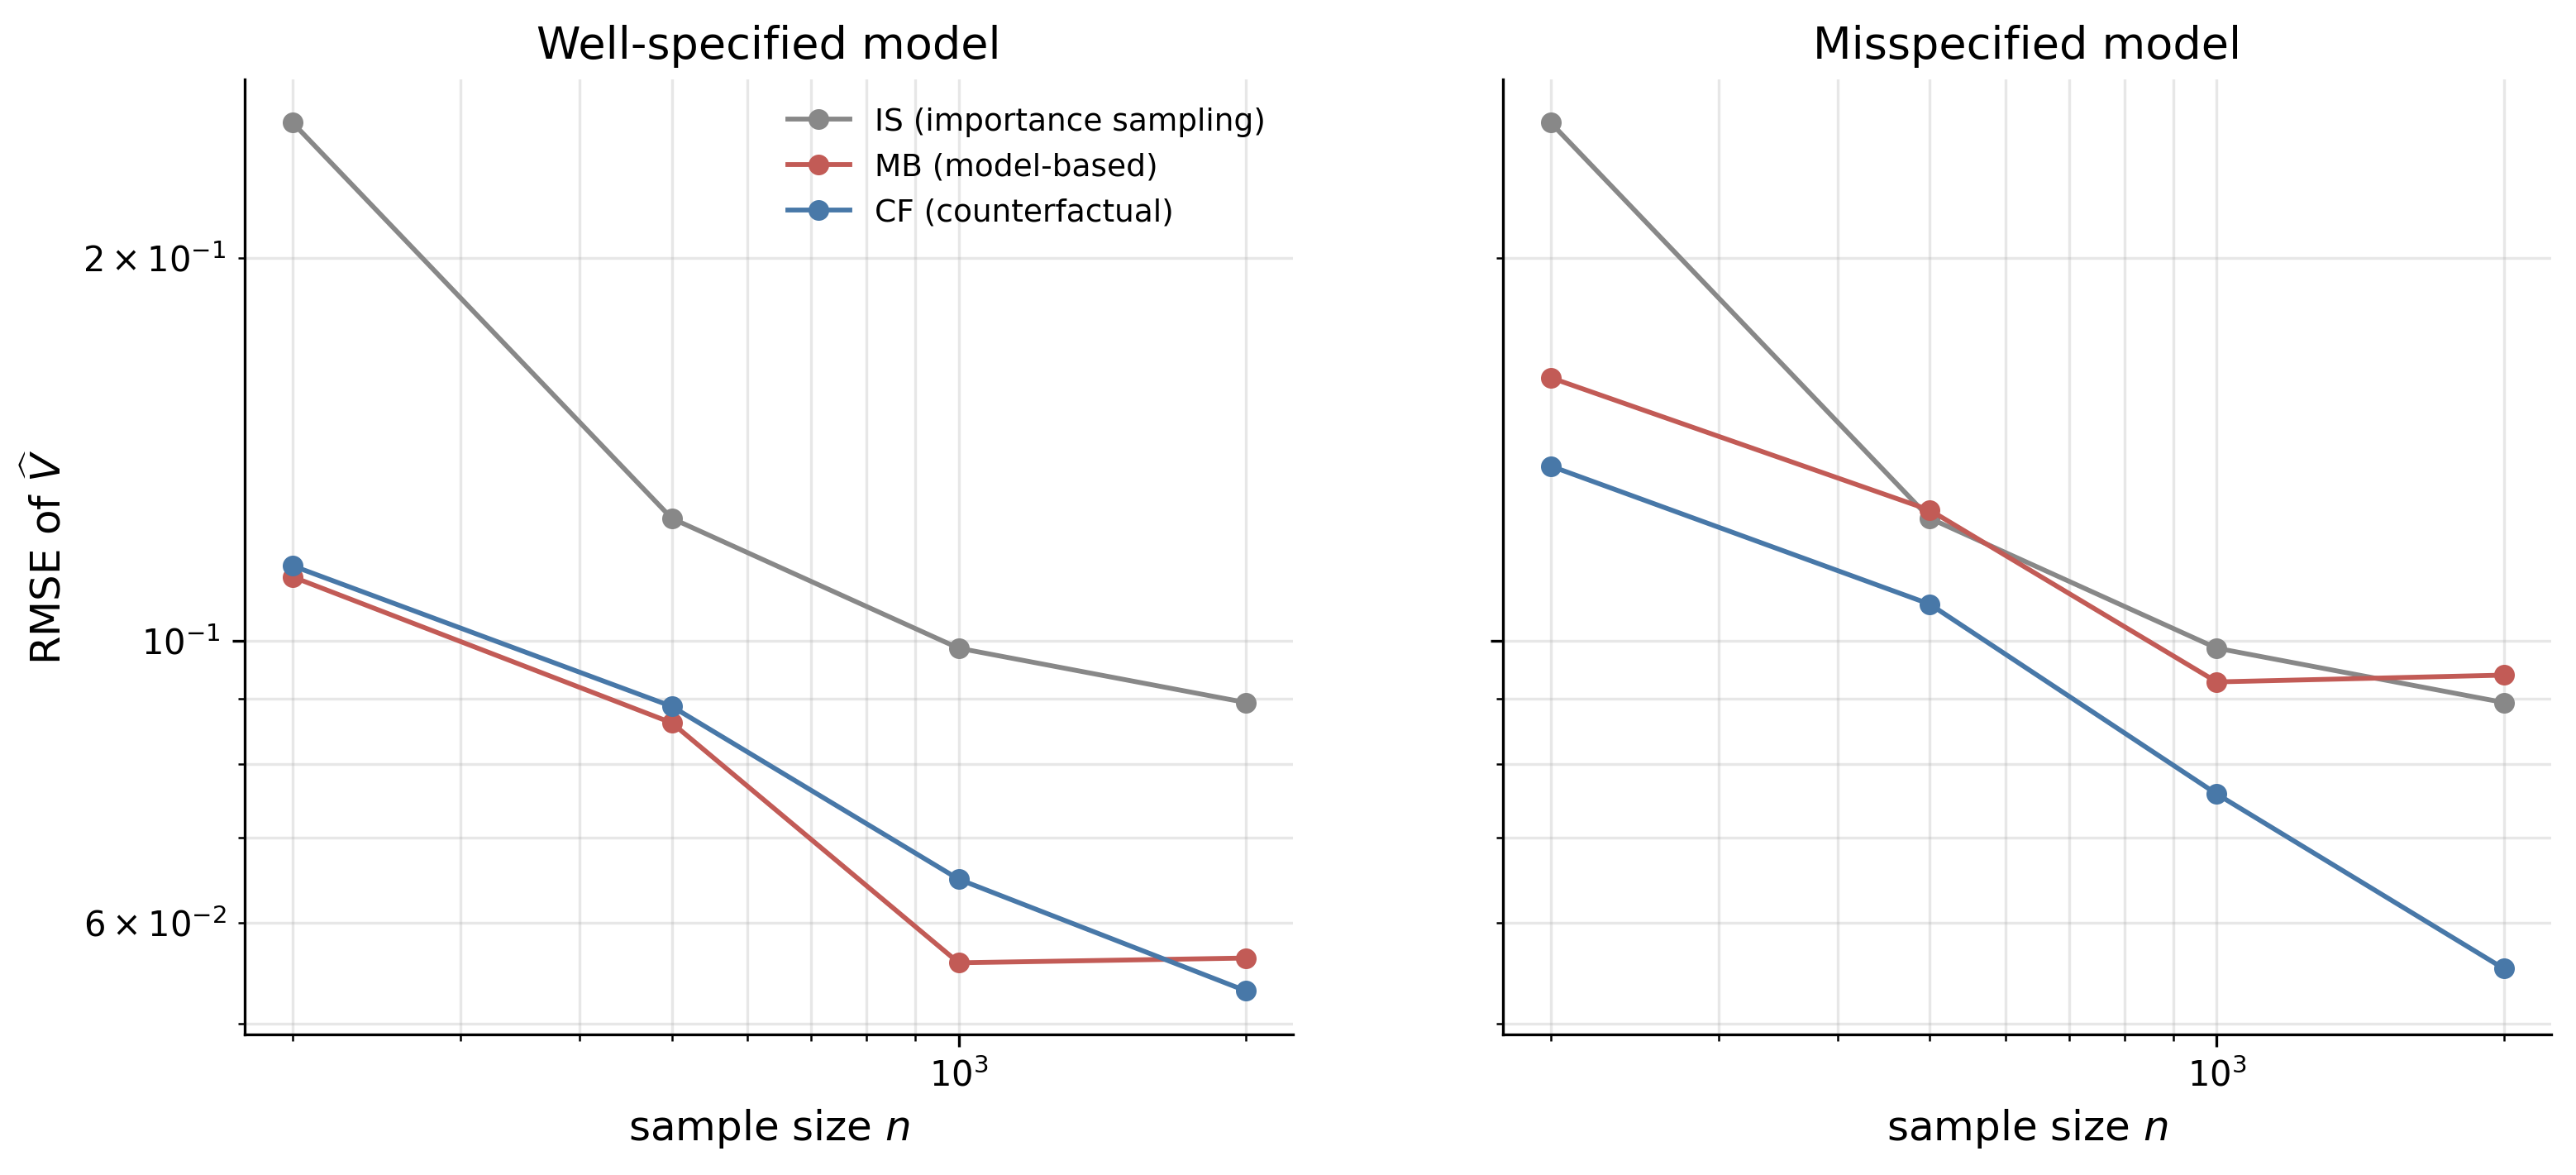
\includegraphics[width=0.85\linewidth]{../ch12_forecasting_rl/sims/counterfactual_ope.png}
\caption{Root mean squared error of three OPE estimators against the
sample size, log-log scale, two panels. Left panel: well-specified
outcome model. Right panel: misspecified model (interaction omitted).
The MB estimator's RMSE plateaus under misspecification as the bias
dominates the variance; the CF estimator's RMSE continues to decline.}
\label{fig:cfope_rmse}
\end{figure}

Table~\ref{tab:cfope_summary} reports bias, standard deviation, and
root mean squared error at $n = 1000$. Under well-specification, the
model-based estimator attains bias $-0.001$ and RMSE $0.056$, the
counterfactual estimator attains bias $0.003$ and RMSE $0.065$, and the
importance-sampling estimator attains bias $0.017$ and RMSE
$0.099$. The MB and CF estimators are statistically indistinguishable
and both improve on IS. Under misspecification, the MB estimator's
bias jumps to $-0.072$ and its RMSE to $0.093$, while the CF
estimator's bias remains at $0.002$ and its RMSE at $0.076$. The CF
estimator's RMSE is $18\%$ lower than MB's, and the bias is two orders
of magnitude smaller. The IS estimator is unchanged across scenarios
because it does not use an outcome model.
Figure~\ref{fig:cfope_rmse} plots RMSE against $n$ on log-log scale.
The MB curve flattens under misspecification at the population bias of
the OLS projection, the CF curve continues to decline at the parametric
rate, and the IS curve traces the higher-variance parametric rate that
the importance-weighted estimator delivers without any model
assistance.

The two simulations of the chapter make the same methodological point
on two different decision structures. The decision-focused AR(1)
forecaster of Section~\ref{sec:forecasting_rl_sim} beats the
prediction-focused OLS forecaster on realised newsvendor cost
precisely when the noise model is misspecified. The counterfactual OPE
estimator above beats the model-based estimator on RMSE precisely when
the outcome model is misspecified. The corrective in both cases is a
training or evaluation objective that knows about the decision-induced
loss, not the marginal forecast loss. The recipe extends naturally to
sequential and to non-stationary settings, where decision-focused
regret bounds at rate $T^{-1/4}$ exist under a margin condition on the
decision polytope \citep{Capitaine2025} and the extension to
action-conditional foundation forecasters remains a research frontier.
